\chapter{Good Practices}
\label{cha:good_practices}

Many common software techniques, processes, and applications were used throughout
cluster implementation to improve overall code quality and to better and easily manage
the Git\footnote{\url{https://git-scm.com}} repository automatically. It would
be virtually impossible to list and explain them all in detail. Also, there are
several guides and publications available on them. Therefore, this attachment
will just briefly cover the two most well-known and widely used techniques that
have been used together, without going into much detail. \\ %
Finally, it is explained how the cluster implementation's final release archive
bundle is generated using a YAML configuration file and a POSIX script.

\section{DevOps}
\label{sec:good_practices_devops}

DevOps is a technique that integrates and automates Software Development (Dev) and
IT Operations (Ops). The combination of cultural philosophies, practices, and
tools improves an organization's capacity to provide applications and services
at high velocity: changing and enhancing products at a quicker rate than traditional
software development and infrastructure management procedures. Implementing a
DevOps paradigm for a project can result in significant benefits such as
increased speed, rapid delivery, reliability, scale, improved collaboration, and
security\cite{devops}. Figure \ref{fig:devops} depicts the cyclical collection of
DevOps phases. Depending on their primary goal, organizations might prioritize different
aspects of the DevOps paradigm.

DevOps is essential in modern software development and is intrinsically linked to
the Continuous Practices discussed in the next section.

\begin{figure}[htbp]
  \centering
  \def\stackalignment{r}\stackunder{ 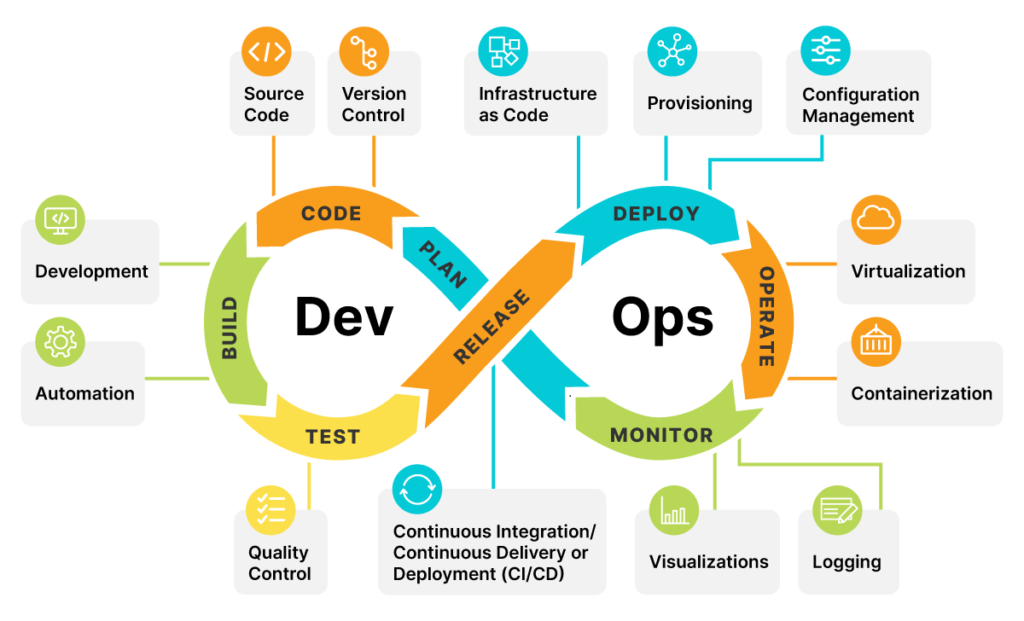
\includegraphics[width=.8\linewidth]{images/attachments/devops.png} } %
  {\scriptsize Source: \url{https://www.edureka.co/blog/what-is-devops} }
  \caption{Cyclical collection of DevOps phases}
  \label{fig:devops}
\end{figure}

\section{Continuous Practices}
\label{sec:continuous_practices}

Continuous Practices also referred to as Continuous Integration, Delivery, and Deployment,
are software development industry strategies that enable organizations to
release new features and products on a regular and consistent basis while
simultaneously keeping the code repository in a consistent state\cite{continuous_practices}.
When a new change is made to the code and pushed to the main repository, it is automatically
checked, compiled, and tested to guarantee code standards, consistency, and that
there are no potentially breaking changes in the prior application's behavior.
The relationship between the three Continuous Practices is depicted in figure
\ref{fig:continuous_practices}.

\begin{figure}[htbp]
  \centering
  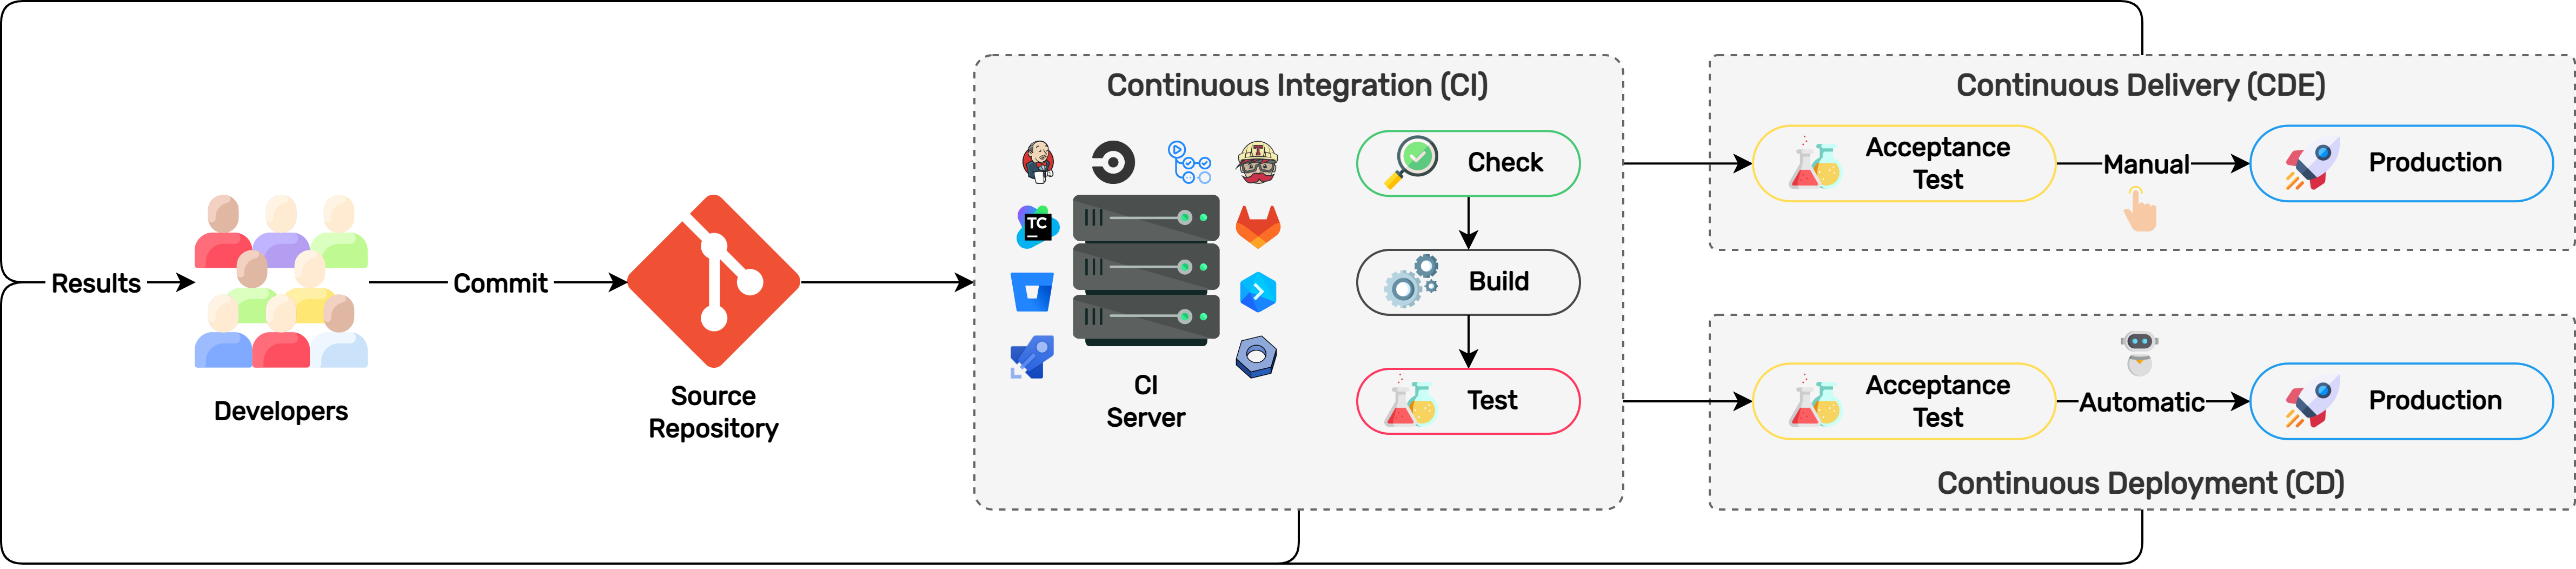
\includegraphics
  [width=.9\linewidth]{images/attachments/continuous_practices.png}
  \caption{Relationship between Continuous Integration, Delivery and Deployment}
  \label{fig:continuous_practices}
\end{figure}

Two automatic workflows to manage Continuous Practices on the source repository have
been implemented in the cluster implementation using GitHub Actions\footnote{\url{https://docs.github.com/actions}}.
The first workflow\footnote{\url{https://github.com/carlocorradini/reCluster/blob/main/.github/workflows/ci.yml}}
executes CI and CDE operations, while the second workflow\footnote{\url{https://github.com/carlocorradini/reCluster/blob/main/.github/workflows/codeql.yml}}
scans the code and generates security alerts if any known security vulnerabilities
are discovered. Furthermore, Dependabot\footnote{\url{https://github.com/dependabot/dependabot-core}}
has been added to keep all project dependencies up to date and to inform when a security
vulnerability is identified on a certain installed version. \\ %
Because of the use of Git Hooks\footnote{\url{https://git-scm.com/book/en/v2/Customizing-Git-Git-Hooks}},
a kind of local CI pipeline that examines every file before committing has also
been developed\footnote{\url{https://github.com/carlocorradini/reCluster/blob/main/.husky/pre-commit}}.
Because it may be skipped with a configuration flag, this procedure does not
substitute a true CI server. \\ %
The previously mentioned CI/CDE workflow fully automates the creation of a new
release\footnote{\url{https://github.com/carlocorradini/reCluster/releases}}. When
a new Git Tag\footnote{\url{https://git-scm.com/book/en/v2/Git-Basics-Tagging}} is
pushed to the main repository and the CI pipeline succeeds, the current cluster
implementation code is bundled (see section \ref{subsec:good_practices_bundle})
and released with the same name as the Git Tag. In the future, a CD pipeline
will be implemented that automatically produces a prerelease anytime a new
change in the code is made, ensuring that the newest nightly code is always available,
even if it is not as stable as a tagged release. \\ %
It should be noted that all prior implementations of Continuous Practices rely
on the GitHub platform. Yet, there are equivalent implementations for
practically every other coding platform.

\subsection{Continuous Integration}
\label{subsec:good_practices_continuous_practices_continuous_integration}

Continuous Integration (CI) is a well-established development process in the software
development industry in which team members regularly integrate and merge development
work (e.g., code). CI allows software organizations to have shorter and more
frequent release cycles, enhance software quality, and raise overall
productivity. This practice involves automated software checking, building and
testing\cite{continuous_practices}.

\subsection{Continuous Delivery}
\label{subsec:good_practices_continuous_practices_continuous_delivery}

Continuous Delivery (CDE) aims to ensure that an application is always ready for
production after passing automated tests and quality checks. CDE leverages a collection
of processes, such as CI and deployment automation, to deliver software automatically
to a production-like environment. This method has various advantages, including fewer
deployment risks, cheaper costs, and faster user feedback. Having a Continuous
Delivery approach necessitates a Continuous Integration process.\cite{continuous_practices}.

\subsection{Continuous Deployment}
\label{subsec:good_practices_continuous_practices_continuous_deployment}

Continuous Deployment (CD) deploys an application to production or customer environments
automatically and continuously. What distinguishes Continuous Deployment from
Continuous Delivery is the presence of a production environment (i.e., actual customers):
the purpose of Continuous Deployment practice is to automatically and consistently
deploy every update into the production environment. It's important to note that
CD practice implies CDE practice, but not the opposite. While the final
deployment in CDE is a manual process, there should be no manual steps in CD,
where changes are pushed to production as soon as developers commit them via a
deployment pipeline. \\ %
CDE is a pull-based approach in which an organization determines what and when
to deploy; CD is a push-based approach. In other words, CDE's scope excludes frequent
and automatic release, and CD is therefore a continuation of CDE. While CDE may be
applied to all kinds of systems and organizations, CD may only be appropriate
for particular types of organizations or systems\cite{continuous_practices}.

\section{Bundle}
\label{sec:good_practices_bundle}

To distribute a release of the cluster implementation, a mechanism that bundles all
required files and directories in a single archive file have been implemented.
The bundle is created automatically by the CDE workflow pipeline and uploaded on
GitHub with the name \texttt{recluster.tag.gz}. The archive file is composed of
a configuration file (see section \ref{subsec:good_practices_bundle_configuration})
that lists all necessary files and directories, and a POSIX script (see section
\ref{subsec:good_practices_bundle_script}) reads the configuration file and generates
the archive file, which may then be published. \\ %
It should be noted that the CDE pipeline is not required to build a bundle. The latter
enables organizations that do not wish to use the workflow to generate a bundle or
to locally test a cluster with a different implementation without involving any workflow.

\subsection{Configuration}
\label{subsec:good_practices_bundle_configuration}

The bundle configuration file, \texttt{bundle.config.yaml}, is written in \texttt{YAML}
format. \\ %
The attributes structure is a mapping that adheres to the development project's
tree hierarchy organization of files and directories\footnote{\url{https://github.com/carlocorradini/reCluster}}.
The key of an attribute is the file or directory name, and the value can be of
two types:
\begin{enumerate}
  \item \texttt{boolean}
    \newline
    The \texttt{true} value indicates that the file or directory should be copied
    (recursively), whereas the \texttt{false} value indicates that the file or directory
    should be ignored.
    \newline
    When the value is \texttt{true} and it is a directory, the included files
    and directories are copied in the order specified by the Git index and
    working tree\footnote{\url{https://git-scm.com/docs/git-ls-files}}.

  \item \texttt{mapping}
    \newline
    Applicable exclusively to a directory (parent), defines a mapping of files and
    directories that are contained in the parent directory.
    \newline
    A special metadata attribute, defined as \texttt{\_\_}, does not reflect a
    directory tree mapping and is instead employed by the script for specific
    operations and management that are applied to the current directory where
    the special attribute is located. At the moment, the only attribute that can
    be defined in the metadata is \texttt{run}, which provides an inline POSIX
    command. When generating the bundle file, all metadata attributes are
    examined and, if a \texttt{run} is identified, it is executed. It should be
    noted that the working directory for \texttt{run} is always the directory containing
    the metadata attribute. If the first two characters are \texttt{./}, the absolute
    path of the project's root directory is substituted. This facilitates the
    execution of scripts from various directories.
\end{enumerate}
Listing \ref{lst:bundle_config} displays the contents of the \texttt{bundle.config.yaml}\footnote{\url{https://github.com/carlocorradini/reCluster/blob/main/scripts/bundle.config.yaml}}
bundle configuration file. It is worth noting the use of the metadata attribute \texttt{\_\_}
in combination with the \texttt{run} attribute for executing applications and/or
programs that provide various outputs required for the release bundle.

\begin{lstlisting}[language=yaml, alsoletter={._-}, morekeywords={[2]{__, run, install.sh, LICENSE, README.md, configs, certs, k3s, k8s, autoscaler, loadbalancer, config.yaml, deployment.yaml, registry, node_exporter, recluster, ssh, dependencies, prometheus, distributions, alpine, arch, logo.png, iso, docs, scripts, certs.sh, configs.sh, configs.config.yaml, server, package.json, package-lock.json, build, prisma, schema.prisma, migrations}}, xleftmargin=\parindent, label={lst:bundle_config}, caption=Content of bundle configuration file]
  __:
    run: "./scripts/inline.sh --in-file ./install.sh --overwrite"
  install.sh: true
  LICENSE: true
  README.md: true

  configs:
    README.md: true
    certs: true
    k3s: true
    k8s:
      README.md: true
      autoscaler: true
      loadbalancer:
        __:
          run: "wget --output-document=deployment.yaml https://raw.githubusercontent.com/metallb
                  /metallb/v0.13.7/config/manifests/metallb-native.yaml"
        config.yaml: true
        deployment.yaml: true
        README.md: true
      registry: true
    node_exporter: true
    recluster: true
    ssh: true

  dependencies:
    __:
      run: "./dependencies/dependencies.sh --sync-force"
    autoscaler: true
    k3s: true
    node_exporter: true
    prometheus: true

  distributions:
    alpine:
      __:
        run: "./distributions/alpine/build.sh"
      README.md: true
      logo.png: true
      iso: true
    arch:
      __:
        run: "./distributions/arch/build.sh"
      README.md: true
      logo.png: true
      iso: true

  docs: true

  scripts:
    __:
      run: "./scripts/inline.sh --in-file ./certs.sh --overwrite && ./scripts/inline.sh --in-file
              ./configs.sh --overwrite"
    README.md: true
    certs.sh: true
    configs.sh: true
    configs.config.yaml: true

  server:
    __:
      run: "npm run build:clean && npm run build"
    README.md: true
    package.json: true
    package-lock.json: true
    build: true
    prisma:
      schema.prisma: true
      migrations: true
\end{lstlisting}

\subsection{Script}
\label{subsec:good_practices_bundle_script}

To automate all bundle-related procedures, a POSIX script named \texttt{bundle.sh}\footnote{\url{https://github.com/carlocorradini/reCluster/blob/main/scripts/bundle.sh}}
is used. Its primary function is to read the bundle configuration file, read
metadata attributes, and generate a bundle archive file containing all files and
directories specified therein. \\ %
The script requires some \texttt{coreutils} package's utility programs and the
\texttt{yq} application to correctly handle \texttt{YAML} file and syntax. \\ %
application. \\ %
The script behavior of the bundle can be changed using parameter flags. The acceptable
setup settings are provided in the table below.

\begin{xltabular}
  {\textwidth} { >{\ttfamily}l | X | >{\ttfamily}c }

  \multicolumn{1}{ c |}{\large{\textbf{Name}}} &
  \multicolumn{1}{ c |}{\large{\textbf{Description}}} &
  \multicolumn{1}{ c }{\large{\textbf{Default Value}}} \\ \hhline{===}

  --config-file <FILE> & Path to the bundle configuration file (\texttt{<FILE>}).
  \newline
  Both relative and absolute paths are supported.
  \newline
  It should be noted that the configuration file name does not have to be \texttt{bundle.config.yaml},
  but may be any name and extension. The sole condition is that it must be in
  \texttt{YAML} format and that the attributes structure is respected. & bundle.config.yaml
  \\ \hline

  --out-file <FILE> & Name of the file path where the generated bundle archive file
  should be saved.
  \newline
  Absolute and relative paths are both supported.
  \newline
  By default, it is saved in the current working directory.
  \newline
  The extension name should always be \texttt{.tar.gz} to distinguish a compressed
  tar archive file. & bundle.tar.gz \\ \hline

  --skip-run & Skip all commands in the metadata attribute \texttt{run}. & false
  \\ \hline

  --log-level <LEVEL> & Logging level (\texttt{<LEVEL>}).
  \newline
  Attachment \ref{cha:logging} provides additional information regarding logging
  and logging levels.
  \newline
  The following logging levels are supported (listed in descending order of
  importance):
  \begin{itemize}[noitemsep]
    \item[\protect\icircled{\texttt{5}}] \texttt{fatal}

    \item[\protect\icircled{\texttt{4}}] \texttt{error}

    \item[\protect\icircled{\texttt{3}}] \texttt{warn}

    \item[\protect\icircled{\texttt{2}}] \texttt{info}

    \item[\protect\icircled{\texttt{1}}] \texttt{debug}
  \end{itemize}
  & info \\ \hline

  --help & Display a help message and terminate (successfully). & \\ \hline

  \caption{Bundle script parameters}
\end{xltabular}

To generate an archive bundle file, named \texttt{recluster.tar.gz}, that contains
all files and directories listed in the configuration file, just execute: \lstinline[language=shell,
alsoletter={.-}, morekeywords={[2]{bundle.sh}}, morekeywords={[3]{--out-file}}]{./bundle.sh --out-file "recluster.tar.gz"}